%===============================================
\chapter{Partition Of Unity}
%===============================================


%===============================================
\section{Constructing A Partition Of Unity}
%===============================================


\begin{figure}
 \centering
 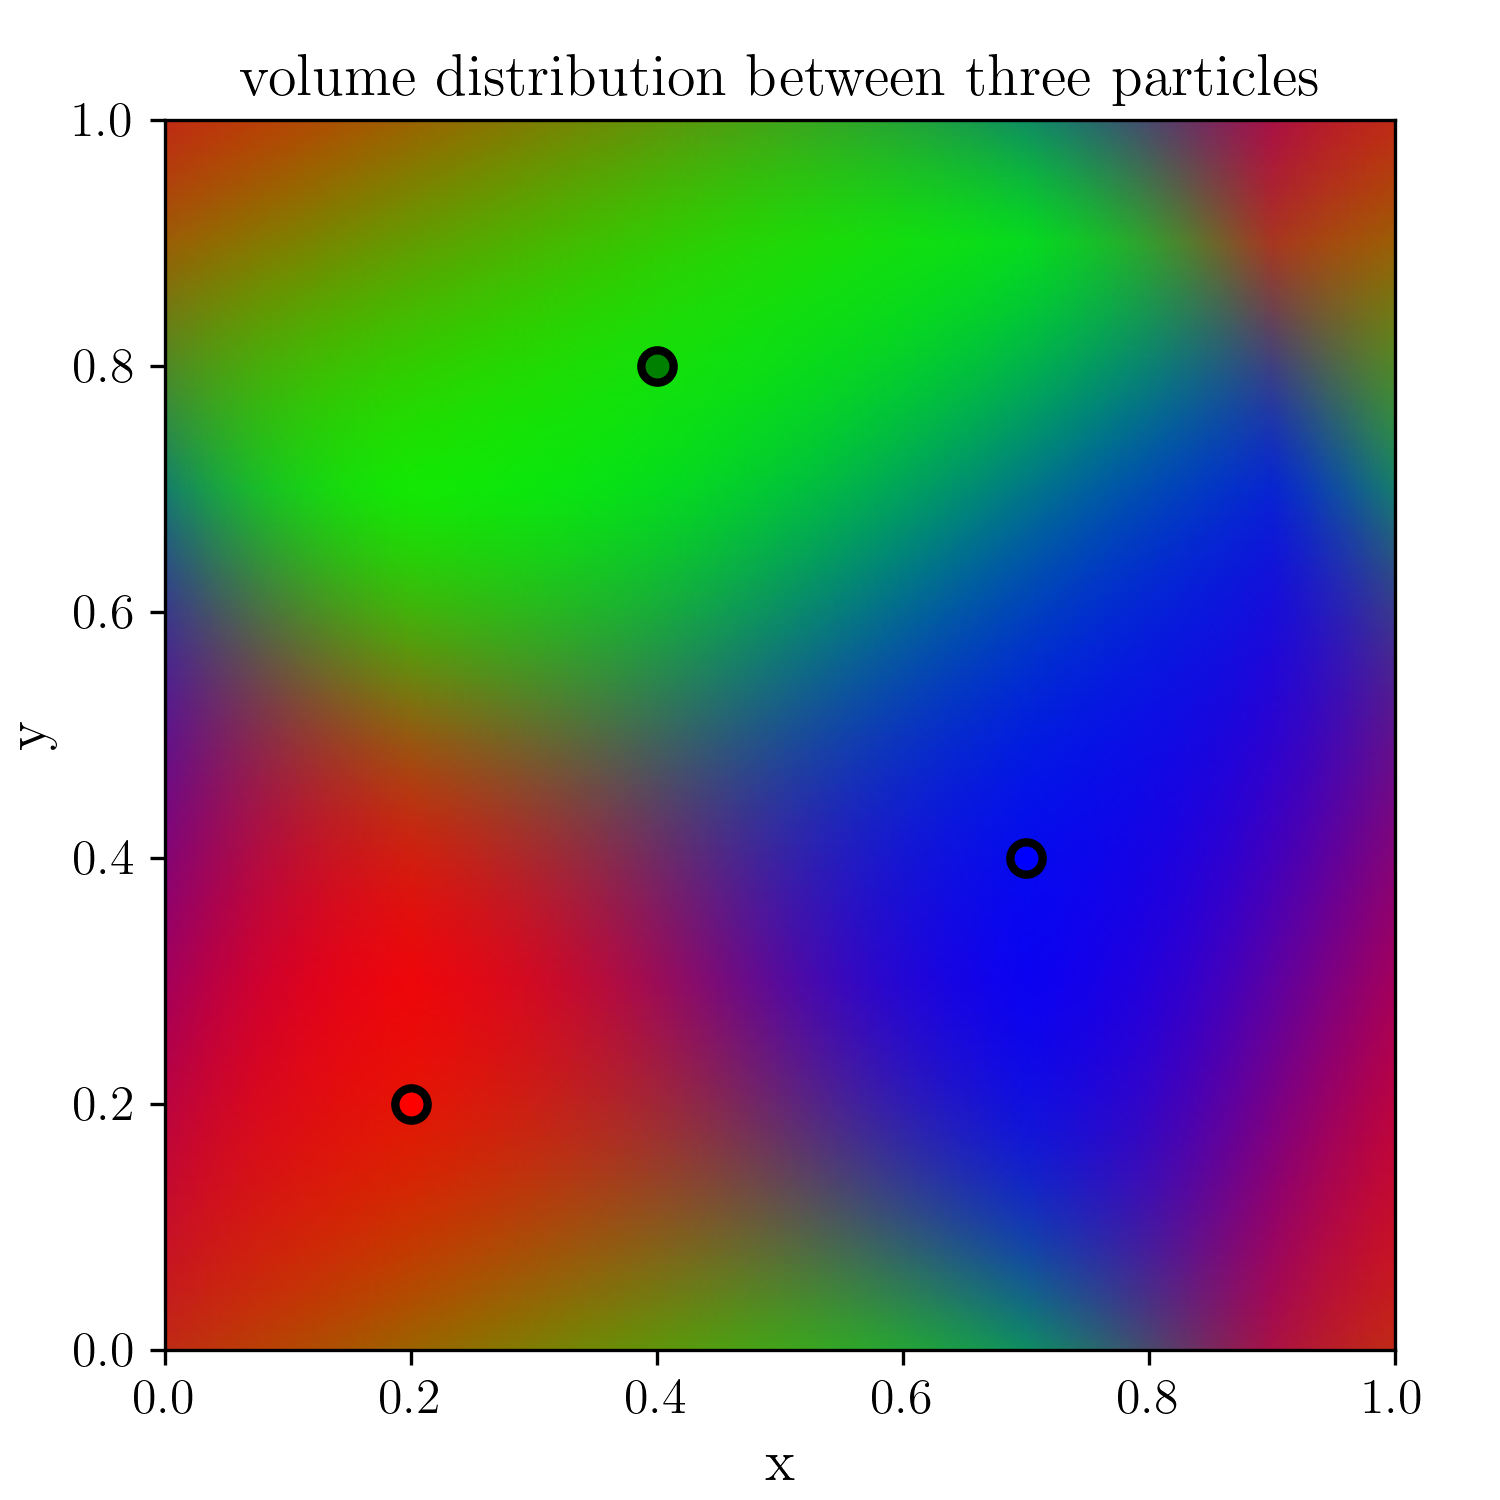
\includegraphics[width=.7\textwidth]{figures/Meshless/volume_distribution_three_particles.png}%
 \caption{
The volume distribution among three particles on a periodic two-dimensional domain with side
length of unity in arbitrary units and periodic boundary conditions. The color at each point of the
domain is determined by assigning RGB values of $\psi$ of the red, green, and blue particle at that
point. Some vertical and horizontal features appear at half the box size's distance from each
particle due to the periodic wrapping: In order for every particle to have a nonzero weight at any
point for this illustrative example, their compact support radii have been chosen to be greater
than half the box size. However this leads to a sharp, non-smooth local minimum in the particle's
weight at that distance in each dimension.
}
\label{fig:psi-volume-distribution}
\end{figure}


A key component in deriving the finite volume particle methods is to make use of a ``partition of
unity'' to distribute the spatial domain among particles, which are used as discretization
elements for the scheme. In a sense, each point in space is ``shared'' among all particles in a
weighted fashion, which will be discussed in detail later. Specifically, at any point $\x$ in space
in the domain, we assign a partition $\psi_i(\x)$ to each particle $i$ such that

\begin{equation}
    \sum_i \psi_i(\x) = 1 \label{eq:partition-of-unity}
\end{equation}

where the sum is assumed to include \emph{all} particles $i$. A visualization of a partition of
unity where a volume is divided among three particles is shown in
Figure~\ref{fig:psi-volume-distribution}. The three particles have been assigned a color red, green,
and blue, respectively. Each point in space is given a color, where the RGB value of the color is
determined by the particle of the corresponding color's contribution to the partition of unity at
that point.

This requirement for the partitions $\psi_i(\x)$ to always sum up to exactly one everywhere is what
lead to the name ``partition of unity''. It can be interpreted as an interpolation technique, where
the real values of a field are distributed among particles and the partition of unity allows the
interpolation at any other point in space (see eq.~\ref{eq:psi-interpolation}).
Condition~\ref{eq:partition-of-unity} can be enforced by choosing $\psi$ to take the following form:

\begin{align}
    \psi_i(\x) &\equiv \frac{1}{\omega(\x)} W(\x, \x_i) \label{eq:psi}\\
    \omega(\x) &= \sum_j W(\x, \x_j) \label{eq:omega}
\end{align}


Where $W(\x, \x_i)$ is in principle some arbitrary function depending on the particle position
$\x_i$. In practice, we want apply some constraints to it motivated by both physical arguments,
mathematical requirements, and computational efficiency. In particular, we want:

\begin{itemize}
 \item As we are going to make use of the derivatives, $W(\x, \x_i)$ shall be continuous and
differentiable, and its first derivative shall also be continuous and differentiable.
 \item $W(\x, \x_i)$ shall be spherically symmetric, i.e. $W(\x, \x_i) = W(|\x - \x_i|)$, to avoid
any preferential direction.
 \item $W(\x, \x_i)$ shall have compact support, i.e. there is some distance $H$ for which
$W(|\x - \x_i| > H) = 0$. $H$ is called the compact support radius. We want to be able to treat the
system locally, and only close-by particles should have an influence on a given point $\x$.
\end{itemize}


Functions that satisfy these demands are well known as ``kernels'' in Smooth Particle
Hydrodynamics methods \citep[e.g.][]{monaghanSmoothedParticleHydrodynamics1992,
priceSmoothedParticleHydrodynamics2012}, and are typically computationally inexpensive
polynomials. For example, throughout this work the cubic B-spline kernel
\citep{monaghanRefinedParticleMethod1985} is used, which is given by

\begin{align}
    q &\equiv \frac{r}{H} \\
    W(\x, H) &= \frac{\sigma}{H^\nu}
        \begin{cases}
            (1 - q)^3 - 4\left(\frac{1}{2} - q \right)^3
                & \text{ if } 0 < q \leq \frac{1}{2} \\
            (1 - q)^3
                & \text{ if } \frac{1}{2} \leq q \leq 1 \\
            0 & \text{ otherwise }
        \end{cases}
    \label{eq:cubic-spline-kernel}
\end{align}

where $\nu$ denotes the number of spatial dimensions, and $\sigma$ is a normalization coefficient
given by

\begin{align}
    \sigma = \frac{8}{3} \text{ for } \nu = 1 &&
    \sigma = \frac{80}{7 \pi} \text{ for } \nu = 2 &&
    \sigma = \frac{16}{\pi} \text{ for } \nu = 3
\end{align}



Table 1 in \cite{dehnenImprovingConvergenceSmoothed2012c} lists some other popular choices for
kernels.

The number of particles that have a non-zero $\psi_i(\x)$  at any $\x$, and thus contribute to the
partition of unity at that point, is determined by the compact support radius $H$. Simultaneously,
the number of particles that contribute to the partition of unity at a given point determines the
accuracy and resolution of the method. Hence it is desirable to demand that (roughly) the same
number of particles is enclosed within the compact support radius at any point. In fact, demanding
a number of neighboring particles to be enclosed within the compact support radius of a given
particle is the criterion which will be used to define the particle's compact support radius. This
will be discussed in more detail in Chapter~\ref{chap:meshless-full}. However, if we want to
maintain a (roughly) equal number of particles having some weight at a given $\x$, then the compact
support radius $H$ can't be a fixed constant which is equal for all particles and for all time.
Instead, it will depend on the current particle configuration, and hence will have a dependence on
the position of evaluation, i.e. $H = H(\x)$.  It is hence appropriate to adapt the notation

\begin{align}
    W(\x, \x_i, H) = W(\x, \x_i, H(\x)) = W_i(\x, H)
\end{align}


Furthermore, it is conventional to talk about the ``smoothing length'' $h$ rather
than the compact support radius $H$ in SPH circles. They are related quantities, with $H \approx
2h$, where the exact value of the proportionality coefficient depends on the kernel choice and
dimension. The reason we use $h$ rather than $H$ is that the smoothing length actually has a direct
physical correspondence: \cite{dehnenImprovingConvergenceSmoothed2012c} have shown that the smoothing
length is directly proportional to the minimal wavelength of a sound wave that can be resolved with
SPH. The exact proportionality coefficients to convert between a smoothing length and the compact
support radius for various kernels and dimensions is given in Table 1 of
\cite{dehnenImprovingConvergenceSmoothed2012c}. To keep the same convention, we'll use the notation

\begin{align}
    W(\x, \x_i, h) = W(\x, \x_i, h(\x)) = W_i(\x, h)
\end{align}


Our demands for the spherically symmetric kernels $W(r)$ to be smooth as well as have compact
support implies that on average they will be a decreasing function of $r$, as they need to go from
some initial value $W(0)$ to zero at $W(r=H)$. Indeed the cubic spline kernel used in this work is
a monotonously decreasing function of distance. This means that each particle's contribution to the
partition of unity is strongest close to the particle position, but it also means that a particle is
likely to be the most dominant contributor to the partition of unity in its immediate vicinity.
This is clearly seen in Figure~\ref{fig:psi-volume-distribution}, where a cubic spline kernel was
used. However, contrary to what the bright red, green, and blue fields close to the particles of
the corresponding color in Figure~\ref{fig:psi-volume-distribution} may suggest, in general no point
in space is assigned to only one particle. The closest particle may be dominant in its
contribution, but not the only contributor to the partition of unity. To underline this point, the
same visualization technique has been applied in Figure~\ref{fig:psi-volume-distribution-vary-h}
for varying smoothing lengths $h$. As $h$ increases, the decline of the kernel value $W_i(r)$
decreases for a specific distance $r$, and the individual particles have more weight at larger
distances. The resulting partition of the volume is much less clearly dominated by any single
particle.


\begin{figure}
 \centering
 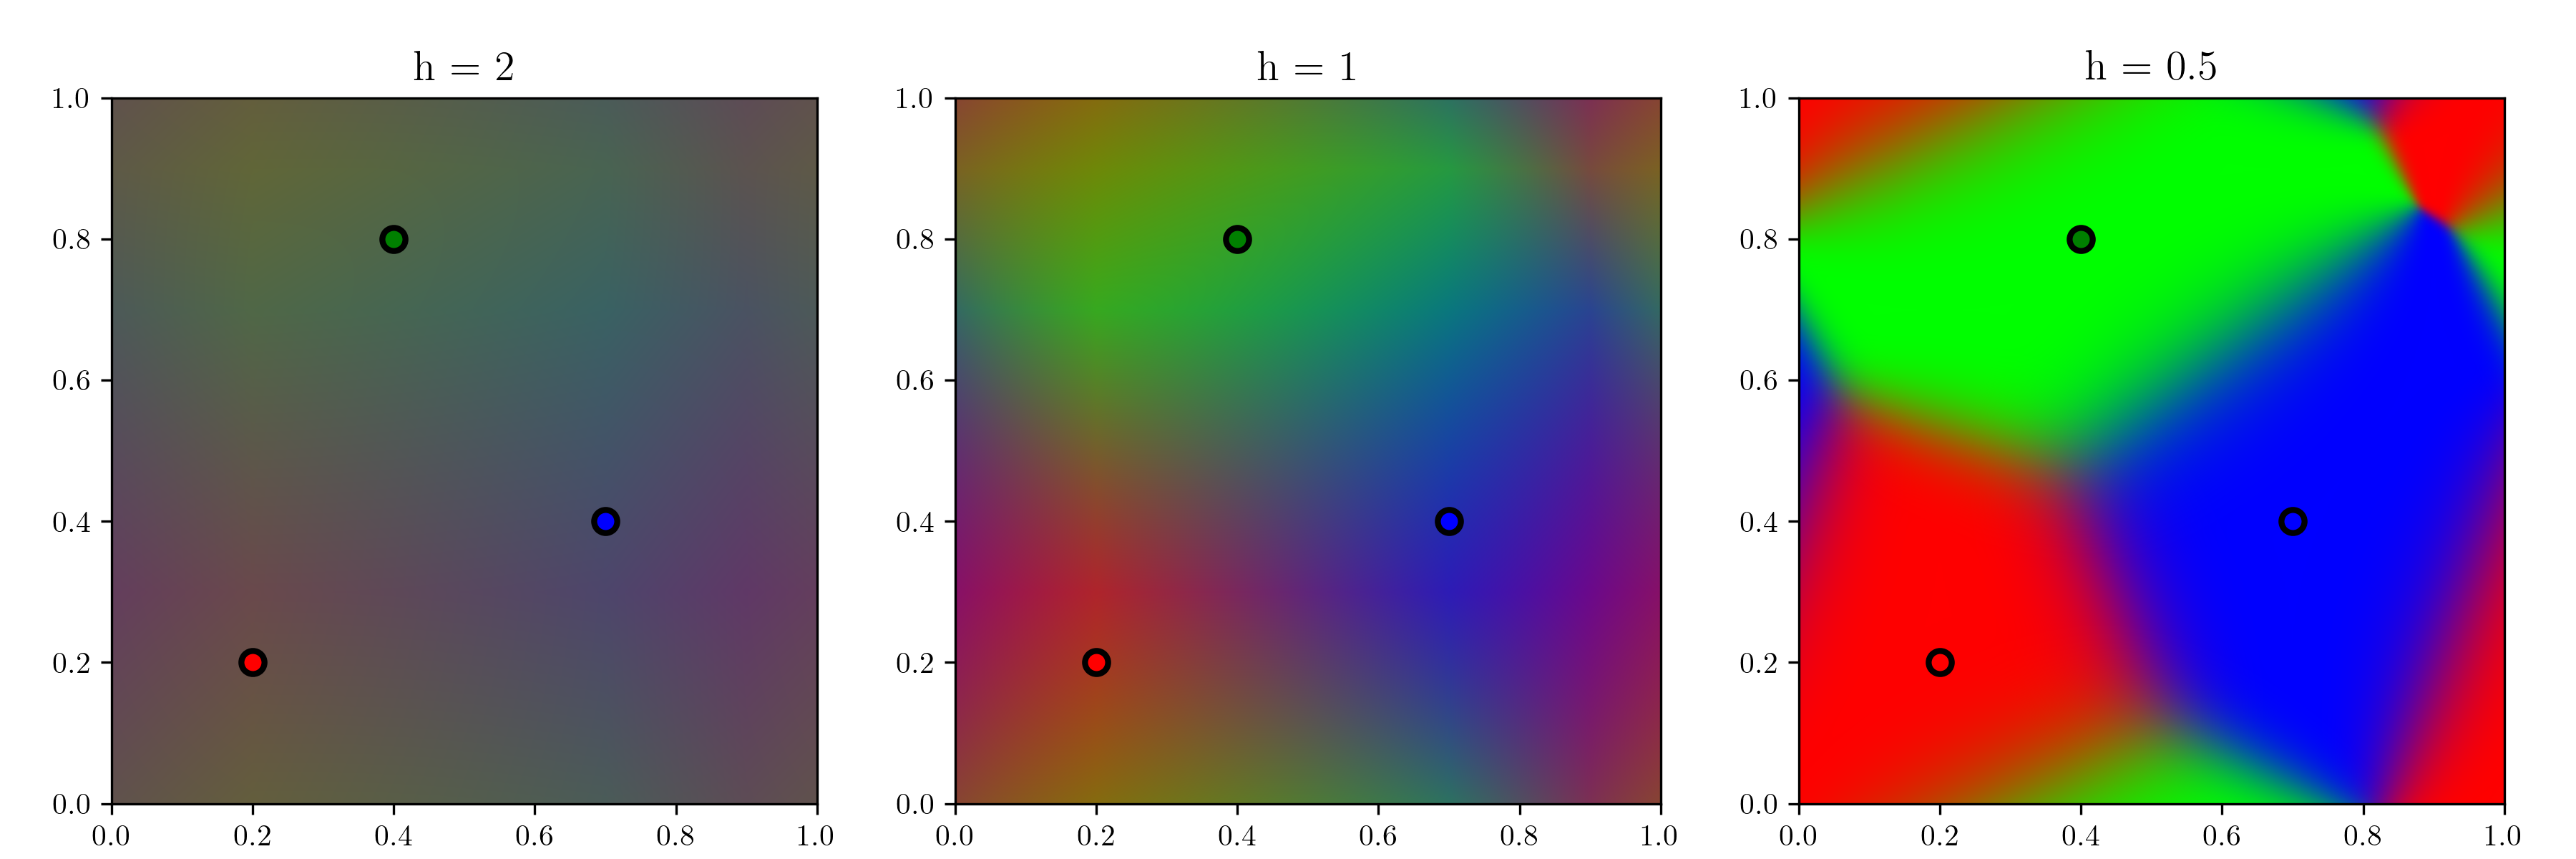
\includegraphics[width=\textwidth]{figures/Meshless/volume_distribution_three_parts_vary_h.png}
 \caption{
Same as Figure~\ref{fig:psi-volume-distribution}, but the volume distributions for three different
smoothing lengths $h = 2$, 1, and 0 are shown. As the smoothing length $h$ increases, the value of
the used cubic spline kernel $W(r)$ increases for a fixed distance $r$, and the relative
contribution to the partition of unity at some given point of particles further away increases
accordingly.
}
\label{fig:psi-volume-distribution-vary-h}
\end{figure}


A further notable point is that even though the kernels $W_i$ are assumed to be spherically
symmetric, the partitions of unity of individual particles, $\psi_i$, in general do not possess the
same symmetry. This is due to the normalization $\omega(\x)$ which depends on the particle
configuration. To illustrate that point, an exemplary partition $\psi_i(\x)$ for a single particle
is shown in Figure~\ref{fig:psi-of-x-contour}.


\begin{figure}
 \centering
 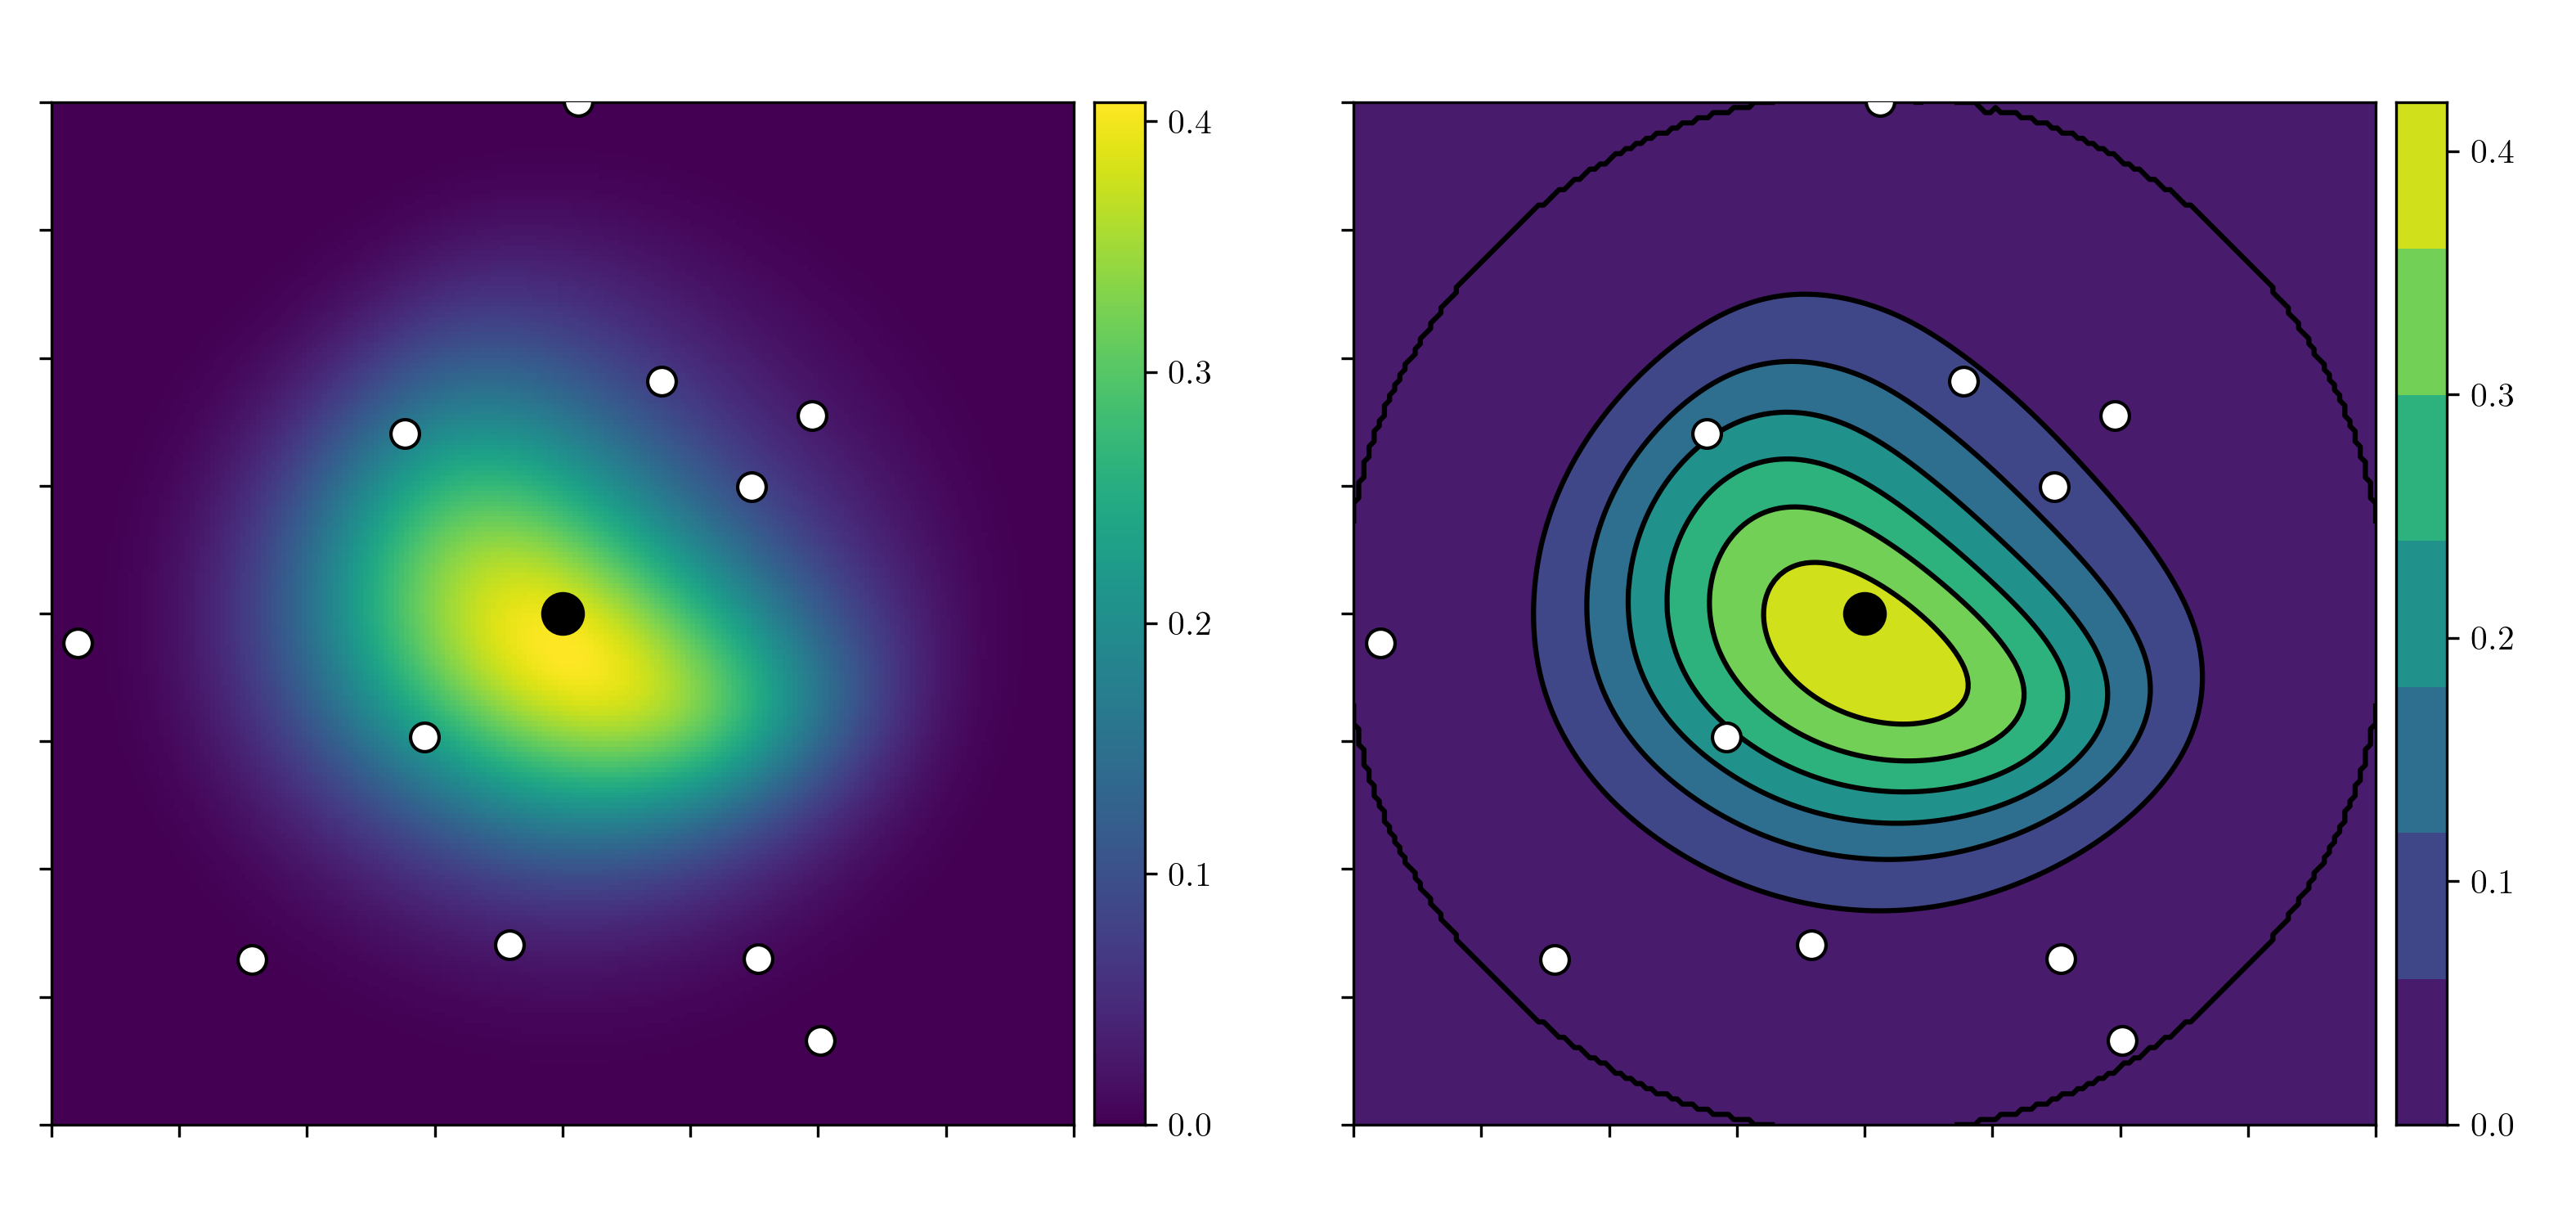
\includegraphics[width=\textwidth]{figures/Meshless/psi_of_x_perturbed.png}
 \caption{ The partition of unity $\psi_i(\x)$ of a single particle (black dot). The left plot
shows the actual values, the right plot shows a contour plot of the same. Even though the used
kernel functions $W$ are spherically symmetric, the resulting partition of unity of a particle
isn't because of the presence of other particles (white dots).
}
\label{fig:psi-of-x-contour}
\end{figure}









%=========================================================
\section{Particle Volume}\label{chap:particle-volume}
%=========================================================


Suppose we have data defined on a set of interpolation points $f_i$, which correspond to function
values at particle positions $\x_i$. Then the interpolated value at some arbitrary $\x$ is given by

\begin{align}
    f(\x) = \sum_i f_i \psi_i(\x) \label{eq:psi-interpolation}
\end{align}

and the gradient is given by

\begin{align}
    \nabla f(\x) = \nabla \left( \sum_i f_i \psi_i(\x) \right) = \sum_i f_i \nabla \psi_i(\x)
\end{align}

since the interpolation points $f_i$ are constant. Using this definition and the volume average of
a function given by

\begin{align}
    V \overline{f} = \int_V f(\x) \de V
\end{align}

we can write

\begin{align}
    V \overline{f}
        = \int_V f(\x) \de V
        = \int_V  \sum_i f_i \psi_i(\x)
        = \sum_i f_i \int_V \psi_i(\x) \de V
        = \sum_i f_i V_i
\end{align}

where

\begin{align}
    V_i \equiv \int_V \psi_i(\x) \de V \label{eq:psi-integral-volume}
\end{align}

are the associated particle volumes.

If we set $f(\x) = f_i = 1$, we obtain

\begin{align}
    V \overline{f} &= V = \sum_i f_i V_i = \sum_i V_i \\
    V &= \sum_i V_i
\end{align}

so by construction, the associated particle volumes conserve the total system's volume in a closed
system.

We can find an expression for the $V_i$ in relation to the kernel function $W(\x, \x_i, h(\x))$. In
what follows, we assume that

\begin{itemize}
    \item $W = W(|\x - \x_i|)$ is symmetric, and
    \item $W$ is normed, i.e. $\int_V W(\x, \x_i, h(\x)) \de V = 1$.
\end{itemize}

We also make use of the following:
%
\begin{enumerate}[label=\roman*.]
\item $f(\x) = \sum_i f(\x_i) \psi_i(\x)$
\item $\psi_i(\x) = \frac{1}{\omega} W(\x - \x_i) = \frac{W(\x - \x_i)}{\sum_j W(\x - \x_j)}$
\item $V_i = \int_V \psi_i(\x) \de V$
\end{enumerate}
%
Then
%
\begin{align}
V_i \
    &\overset{(i)}{=} \ \sum_j \psi_j(\x_i) V_j
    \overset{(iii)}{=} \ \sum_j \psi_j (\x_i) \int_V \psi_j(\x) \de V \\
    &\overset{(ii)}{=} \ \sum_j \frac{W(\x_i - \x_j)}{\sum_k W(\x_i - \x_k)} \int_V \psi_j(\x) \de
V \\
    &= \frac{1}{\sum_k W(\x_i - \x_k)}  \sum_j W(\x_i - \x_j) \int_V \psi_j(\x) \de V \\
    &= \frac{1}{\sum_k W(\x_i - \x_k)}  \sum_j \int_V W(\x_i - \x_j) \psi_j(\x) \de V \\
    &= \frac{1}{\omega(\x_i)}  \sum_j \int_V W(\x_i - \x_j) \psi_j(\x) \de V \\
    &\overset{(i)}{=} \
        \frac{1}{\omega(\x_i)}\underbrace{\int_V W(\x_i - \x) \de V}_{=1 \text{, normalized}} \\
    &= \frac{1}{\omega(\x_i)} \label{eq:particle-volume-exact}
\end{align}

Expression~\ref{eq:particle-volume-exact} is only valid assuming that the
interpolation~\ref{eq:psi-interpolation} and the volume integral

\begin{align}
    \int_V f(\x) \de V = \sum_i f_i V_i \label{eq:psi-volume-integral-step}
\end{align}

are exact, which in general they are not. As will be shown below, the volume integral is
$\order(h^2)$ accurate, giving us

\begin{align}
    V_i = \frac{1}{\omega(\x_i)} + \order(h^2) \label{eq:particle-volume}
\end{align}

To demonstrate the accuracy of the integral~\ref{eq:psi-volume-integral-step}, we multiply the
integrand by $1 = \sum_i \psi_i(\x)$ (which is exact by construction) and use a Taylor expansion
around $\x = \x_i$:

\begin{align}
    \int_V f(\x) \de V
        &= \int_V f(\x) \underbrace{\sum_i \psi_i(\x)}_{= 1} \de V
        = \sum_i \int_V f(\x) \psi_i(\x) \de V \\
        &= \sum_i \left[
            f(\x_i) + (\x - \x_i)\nabla f(\x_i) + \order(\x - \x_i)^2
            \right] \psi_i (\x) \\
        &= \sum_i f(\x_i) \int_V \psi_i(\x) \de V +
            \underbrace{\sum_i \int_V (\x - \x_i) \nabla f(\x_i) \psi_i(\x) \de V}_{=0 \text{, will
be shown later}} + \order((\x - \x_i)^2) \label{eq:integral-psi-interemediate}\\
        &= \sum_i f(\x_i) \int_V \psi_i(\x) \de V + \order((\x - \x_i)^2)
\end{align}


So the integral is $\order((\x - \x_i)^2)$ accurate. Considering that the kernels we use have a
compact support radius $H$ which determine the maximal distance $\x - \x_i$ from a particle at
which the kernel value and hence the partition of unity $\psi_i(\x)$ is non-zero, we can express
the error term using $H$ as the upper boundary for the error, i.e. $\max_i (\x - \x_i) = \max_i H_i
= \max_i H(\x_i)$. Equivalently, since the smoothing length $h$ is directly proportional to $H$, we
might just as well express the error in terms of $h$, and write $\order((\x - \x_i)^2) =
\order(h^2)$ like in eq.~\ref{eq:particle-volume}.

It remains to show that the integral of the first order term in
eq.~\ref{eq:integral-psi-interemediate} is indeed zero. Since the gradient term is evaluated at a
fixed $\x_i$, we can write

\begin{align}
    \sum_i \int_V (\x - \x_i) \nabla f(\x_i) \psi_i(\x) \de V =
    \sum_i \nabla f(\x_i)  \int_V (\x - \x_i)\psi_i(\x) \de V
\end{align}

and it suffices to show that

\begin{align}
    \int_V (\x - \x_i)\psi_i(\x) \de V = 0
\end{align}

For simplicity, we demonstrate this only for the one dimensional case. The extension to several
dimensions is straightforward. Furthermore, we set the integration boundaries to be $(-L, L)$,
where $L$ may be infinity.\footnote{In case $L$ isn't infinity, we ignore for now what happens with
particles which are close enough to the borders $\pm L$ such that the border is within its compact
support radius.} The integral in one dimension is then

\begin{align}
    \int_{-L}^{L} (x - x_i) \psi_i(x) \de x
    = \int_{-L}^{L} (x - x_i) \psi(x - x_i) \de x
    = \int_{-L+x_i}^{L+x_i} s \psi(s) \de s
 \end{align}

where first equality makes use of the other notation for $\psi$, and the last equality follows from
using the substitution $s = x - x_i$. We can now integrate by parts and show that the integral
evaluates to zero:

\begin{align}
    \int_{-L+x_i}^{L+x_i} s \psi(s) \de s &=
    \left[
        s \underbrace{\int_{-L+x_i}^{L+x_i} \psi(s) \de s}_{=\int_{-L}^{L} \psi_i(x) \de x = V_i }
    \right]_{s = -L+x_i}^{L+x_i} -
    \int_{-L+x_i}^{L+x_i} \left[
    \underbrace{\frac{\del}{\del s} s}_{= 1}
    \underbrace{\int_{-L+x_i}^{L+x_i} \psi(s) \de s}_{= V_i} \right] \de s \\
%
    &= \left[ s V_i \right]_{s = -L+x_i}^{L+x_i} - \int_{-L+x_i}^{L+x_i} V_i \de s
    = \left[ s V_i  - s V_i \right]_{s = -L+x_i}^{L+x_i} = 0
\end{align}



Using the partitions of unity, we can now derive concrete expressions for finite volume particle
methods. The partitions of unity will be applied to discretize the conservation laws we want to
solve onto particles.
